\documentclass{article}
	\usepackage[utf8]{inputenc}
	\usepackage{geometry}[top=1cm, right=1cm, left=1cm]
	\usepackage{graphicx}
    \usepackage{tabularx}
	\usepackage{float}
	\title{Solving Flow Free as a \\ Constraint Satisfaction Problem}
	\author{Trent Baker, Dylan Wickham}

\begin{document}

\maketitle

% this might work better as one section instead of subsections. There isn't a TON to say about each individually
\section{Formulating Flow Free as a CSP}
    \subsection{Variables}
        For Flow Free to work as a CSP, each tile must be a variable. Each variable is assigned a color, but has some associated metadata that allows us to structure the problem in an efficient way. For example, to enable us to easily check constraints, each tile is aware of its four neighbors north, east, south and west.
    
    \subsection{Domain}
        The domain for each puzzle is different because it is dynamically generated from the input files. Each node could be assigned to any color that exists in the input, but would be invalid if the assigned color was not in the set of input colors.
    
    \subsection{Constraints}
        While it may seem complicated, the constraints for Flow Free can be simplified into a few relatively simple checks. If a node is assigned a color from the input, it is marked as a source because these are the only nodes that may have exactly one neighbor of the same color. Each other node must have exactly two neighbors of the same color in the final solution. By checking these constraints, we can ensure that there is no ``zig-zagging'' and that all of the paths eventually become contiguous.

\section{Implemented Algorithms}
\subsection{Naive Backtracking Search}
    The Naive Backtracking search can be broken down into three primary parts, selection, assignment, and constraint checking. First, an unassigned node is selected from the set of unassigned nodes remaining in the puzzle. That node is then assigned a possible value from the domain and its neighbors are checked against the constraints described above. If any neighbor does not satisfy all of the constrains, that assignment is invalid and the algorithm will try another possible domain value. If every possible domain value results in an invalid state, then the algorithm will backtrack and attempt different values from the domain for previously assigned nodes.
    % non-obvious implementation choices
    % parameter settings
    % tips for good performance
    

% Not sure about the name for this alg. could just call it smart search.
\subsection{Smart Backtracking Search}
    To add a level of intelligence to our algorithm, we select an unassigned variable by using a heuristic that measures how constrained that node is. This simple change allows the algorithm to realize that it has created an invalid state more quickly. As a consequence however, the set of unassigned nodes must be sorted before each assignment is attempted. For different problems, this technique could be very effective, but when applied to puzzles such as the 9x9maze, this overhead actually causes the algorithm to take longer to complete.
    
    Because the nodes are ordered by their location prior to being sorted, that order is preserved within each value of constrainedness. If the list is shuffled before being sorted, the selection becomes more stochastic while still selecting a node likely to prove the assignment invalid. This also adds to the overhead that slows down the selection process. In our testing, this was not beneficial to performance because nodes not near other recently assigned nodes may not invalidate an assignment for many iterations despite being obviously incorrect to a human observer.
    % non-obvious implementation choices
    % parameter settings
    % tips for good performance

    
\section{Results}
    We measured our algorithms performance in many places. The first puzzle to be solved consistently has unusually long times for importing and rendering. This is likely due to things like setting up internal things such as file system access and loading the image processing libraries into memory. We tested the mazes in different orders and the solve times are similar regardless. Because the importing and rendering are not relevant to the algorithm performance, we have chosen to leave these values as reported by the system.
    
    Due to the nature of the problem, there is exactly one possible assignment that has every node assigned and does not violate any constraints. Because the resulting images are identical for both algorithms, we have only included one set of solutions.
    
    \begin{figure}
	\centering
	\begin{tabularx}{\textwidth}{X X}
		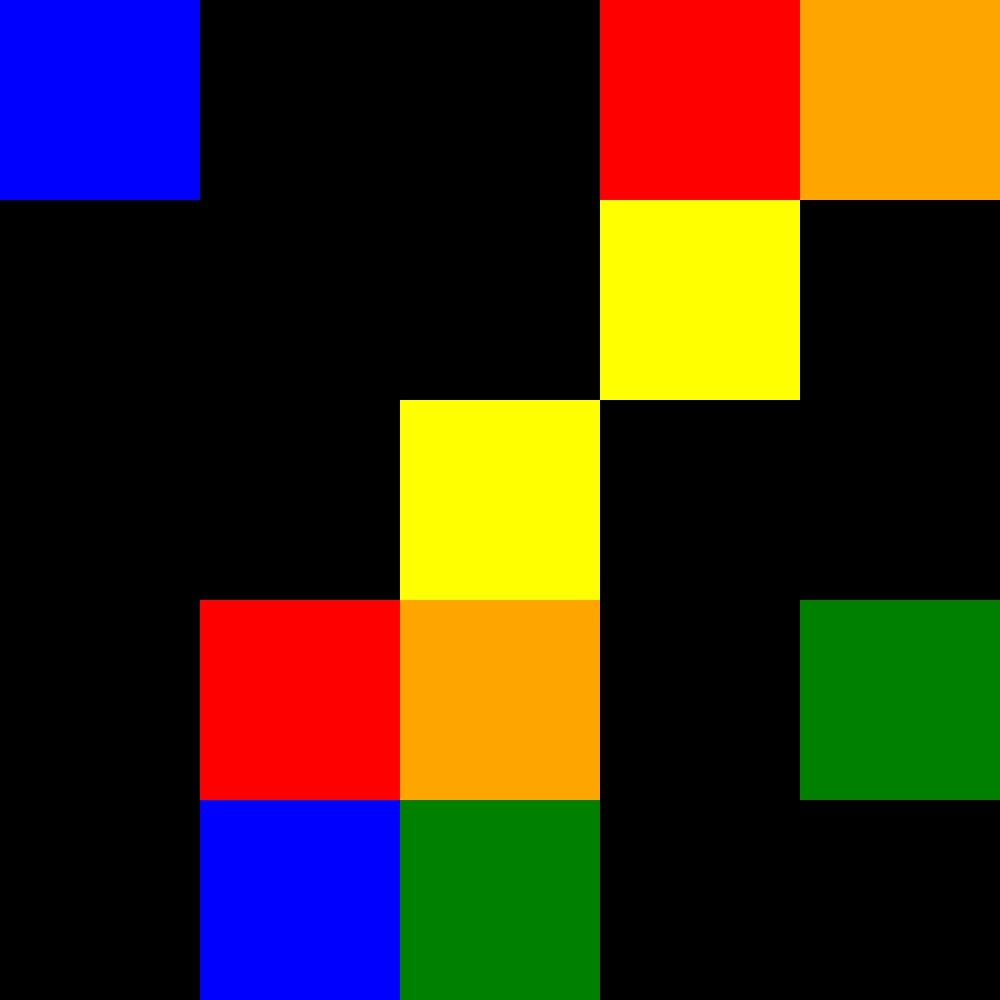
\includegraphics[width=0.4\textwidth]{5x5_input.png} &
		
\includegraphics[width=0.4\textwidth]{5x5_output.png} \\
		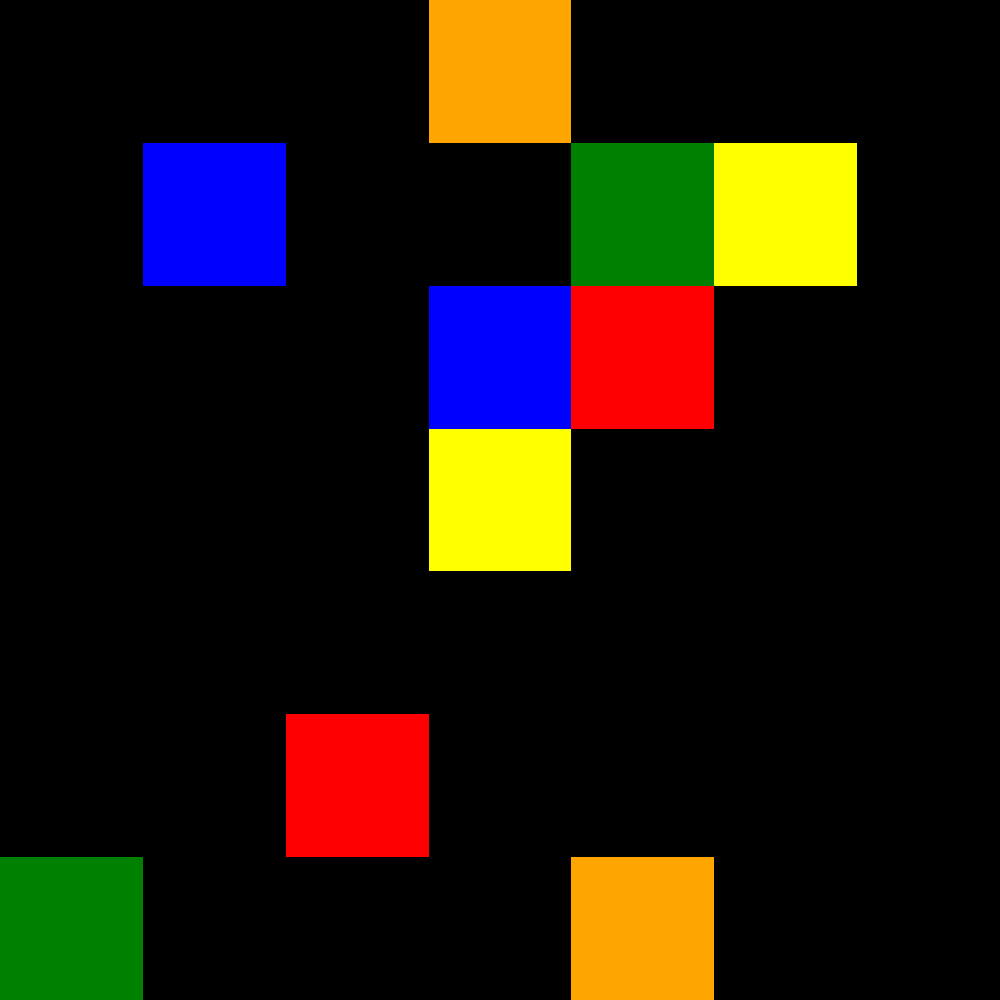
\includegraphics[width=0.4\textwidth]{7x7_input.png} &
		
\includegraphics[width=0.4\textwidth]{7x7_output.png} \\
		
\includegraphics[width=0.4\textwidth]{8x8_input.png} &
		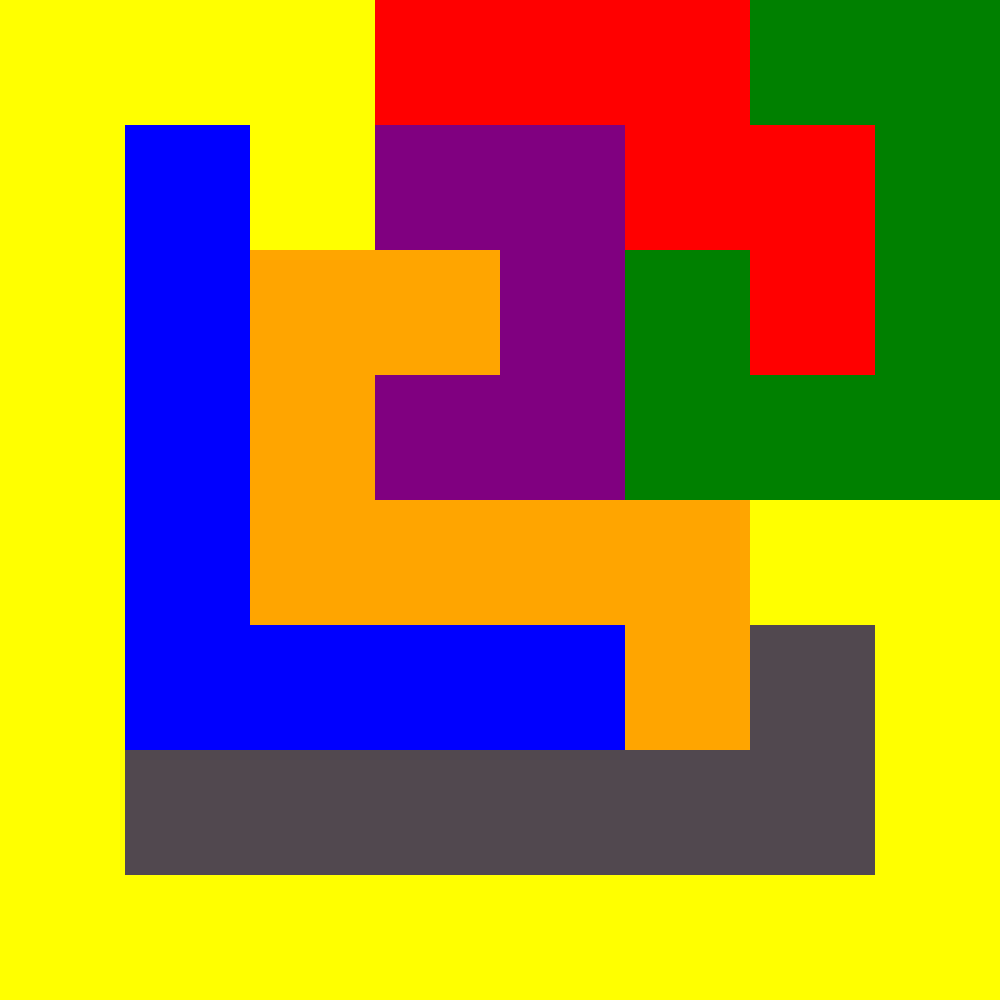
\includegraphics[width=0.4\textwidth]{8x8_output.png} \\
	\end{tabularx}
	\caption{Results for puzzles 5-8}
	\label{fig:resultsA}
\end{figure}
\begin{figure}
	\centering
	\begin{tabularx}{\textwidth}{X X}
		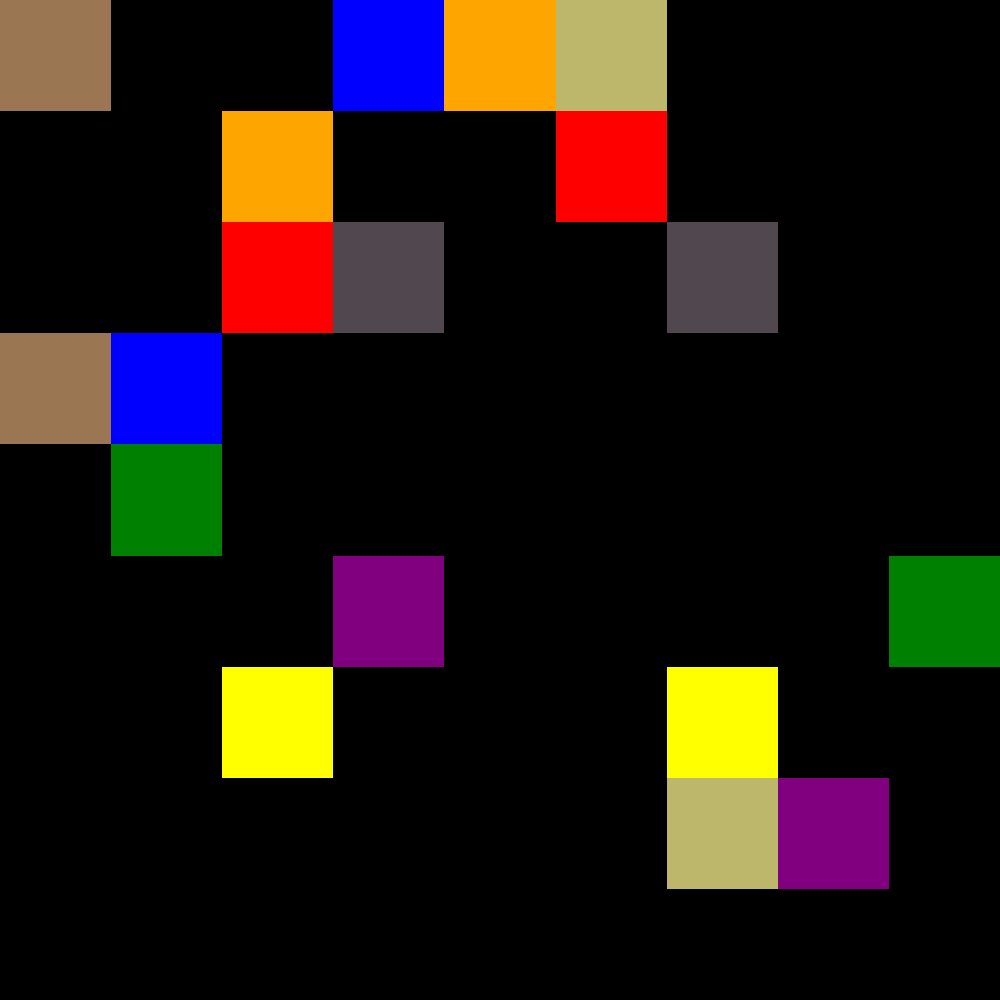
\includegraphics[width=0.4\textwidth]{9x9_input.png} &
		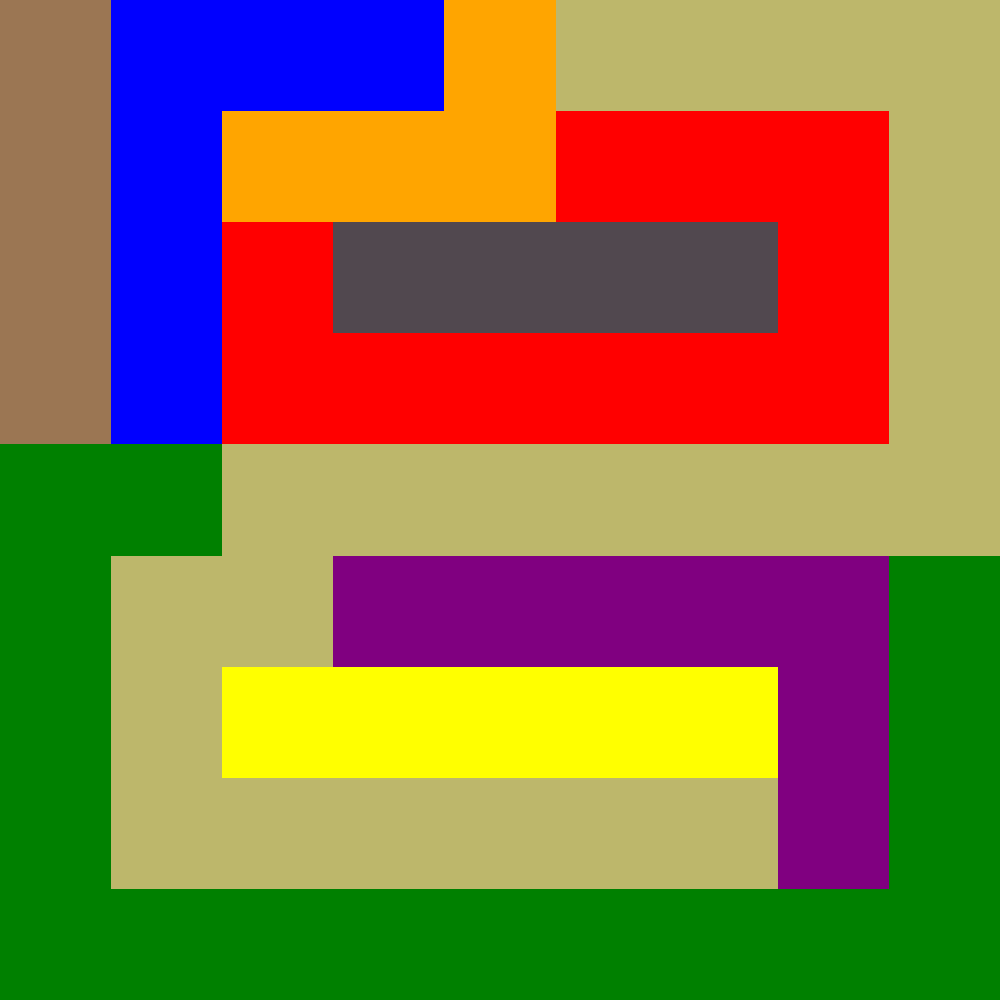
\includegraphics[width=0.4\textwidth]{9x9_output.png} \\
		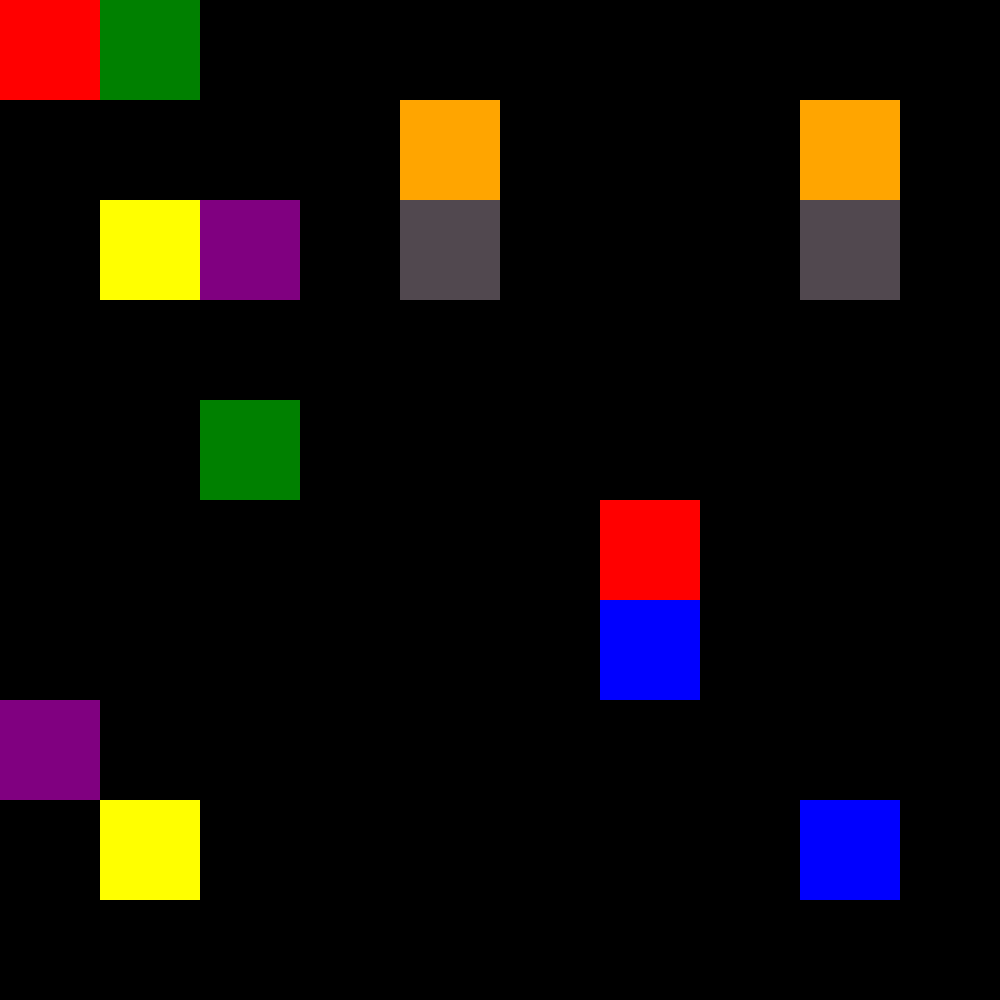
\includegraphics[width=0.4\textwidth]{10x10_input.png} &
		
\includegraphics[width=0.4\textwidth]{10x10_output.png} \\
		
\includegraphics[width=0.4\textwidth]{12x12_input.png} &
		
\includegraphics[width=0.4\textwidth]{12x12_output.png} \\
	\end{tabularx}
	\caption{Results for puzzled 9-12}
	\label{fig:resultsB}
\end{figure}
            
    
    \begin{itemize}
        \item Input - The file that contains the puzzle
        \item Import - The time that our program takes to convert the text input to a 2-D array of nodes
        \item First Render - The time to render and save the starting state of the puzzle before any modifications are made
        \item Solve - The time the algorithm takes to solve the puzzle from start to finish
        \item Assignments - The total number of assignments attempted during the solve
        \item Second Render - The time taken to render and save the completed puzzle
    \end{itemize}

    % for each alg.
    %     rendered solution
    %     number of attempted variable assignments
    %     execution time
\subsection{Naive Backtrack Results}
    \begin{tabular}{c c c c c c}
        Input & Import & First Render & Solve & Assignments & Second Render \\
        \hline
        10x10maze & 43ms & 368ms & 2929ms & 869549 & 14ms \\
        12x12maze & 6ms & 31ms & 4715ms & 5836919 & 8ms \\
        5x5maze & 1ms & 7ms & 1ms & 168 & 7ms \\
        5x5solutionmaze & 1ms & 7ms & 0ms & 0 & 7ms \\
        7x7maze & 0ms & 8ms & 1ms & 1631 & 7ms \\
        8x8maze & 1ms & 8ms & 3ms & 6934 & 8ms \\
        9x9maze & 0ms & 7ms & 91ms & 200021 & 8ms \\
    \end{tabular}   

\subsection{Smart Backtracking Results}
    \begin{tabular}{c c c c c c}
        Input & Import & First Render & Solve & Assignments & Second Render \\
        \hline
        10x10maze & 63ms & 239ms & 1100ms & 726651 & 4ms \\
        5x5maze & 4ms & 1ms & 0ms & 48 & 2ms \\
        5x5solutionmaze & 3ms & 2ms & 0ms & 0 & 4ms \\
        7x7maze & 3ms & 3ms & 4ms & 1266 & 5ms \\
        8x8maze & 4ms & 3ms & 5ms & 2937 & 11ms \\
        9x9maze & 6ms & 38ms & 799ms & 941477 & 2ms \\
    \end{tabular}

\section{Conclusion}
Overall, the Smart Backtracking Algorithm seems better than Naive Backtracking Algorithm as the smart approach almost always requires less assignments and less time to solve the puzzle. The notable exception is the 9x9 maze, however, that seems like an input that just happens to do poorly with smart algorithm and that the mazes in general seem to be solved fasted by the smart algorithm. It appears that the small amount of extra computation done for the smart algorithm has significant benefits.

\section{Individual Contributions}
    \subsection{Trent}
        I adapted some of the code from the previous assignment to work for this project. Because of the problem structure, we could use a decent amount of the code we already wrote. Specifically, the Node class, rendering and importing algorithms could be used with relatively little modification. Dylan wrote the Naive algorithm, and by refactoring into an interface, I created the Smart algorithm that uses much of the same code. I added timers to measure real-time performance, but Dylan added the code to count the number of assignments.
        
    \subsection{Dylan}
        I developed the naive backtracking algorithm. From there, it was refactored by Trent to put shared functionality in the interface. After that, I updated the algorithms to track the number of assignments made. Additionally, made updates to allow for updating the puzzle path, output path, or which algorithm was being used via command line arguments.

\end{document}
